\documentclass[letterpaper,10pt]{article}

\usepackage{enumitem}
\usepackage{titling}
\usepackage{listings,listings-rust}
\usepackage{url}
\usepackage{soul}
\usepackage{hyperref}
\usepackage{setspace}
\usepackage{subfig}
\usepackage{sectsty}
\usepackage{pdfpages}
\usepackage{colortbl}
\usepackage{multirow}
\usepackage{multicol}
\usepackage{relsize}
\usepackage{amsmath}
\usepackage{wasysym}
\usepackage{fancyvrb}
\usepackage[yyyymmdd]{datetime}
\usepackage{amsmath,amssymb,amsthm,graphicx,xspace}
\usepackage[titlenotnumbered,noend,noline]{algorithm2e}
\usepackage[compact]{titlesec}
\usepackage{XCharter}
\usepackage[T1]{fontenc}
\usepackage[scaled]{beramono}
\usepackage[normalem]{ulem}
\usepackage{booktabs}
\usepackage{tikz}
\usetikzlibrary{arrows.meta,automata,shapes,trees,matrix,chains,scopes,positioning,calc,decorations.pathreplacing}
\tikzstyle{block} = [rectangle, draw, fill=blue!20, 
    text width=2.5em, text centered, rounded corners, minimum height=2em]
\tikzstyle{bw} = [rectangle, draw, fill=blue!20, 
    text width=4em, text centered, rounded corners, minimum height=2em]

\definecolor{namerow}{cmyk}{.40,.40,.40,.40}
\definecolor{namecol}{cmyk}{.40,.40,.40,.40}
\renewcommand{\dateseparator}{-}

\let\LaTeXtitle\title
\renewcommand{\title}[1]{\LaTeXtitle{\textsf{#1}}}

\lstset{basicstyle=\footnotesize\ttfamily,breaklines=true}

\newcommand{\CPP}{C\nolinebreak\hspace{-.05em}\raisebox{.4ex}{\tiny\bf +}\nolinebreak\hspace{-.10em}\raisebox{.4ex}{\tiny\bf +}}
\def\CPP{{C\nolinebreak[4]\hspace{-.05em}\raisebox{.4ex}{\tiny\bf ++}}}

\newcommand{\handout}[5]{
  \noindent
  \begin{center}
  \framebox{
    \vbox{
      \hbox to 5.78in { {\bf ECE459: Programming for Performance } \hfill #2 }
      \vspace{4mm}
      \hbox to 5.78in { {\Large \hfill #4  \hfill} }
      \vspace{2mm}
      \hbox to 5.78in { {\em #3 \hfill \today} }
    }
  }
  \end{center}
  \vspace*{4mm}
}

\newcommand{\lecture}[3]{\handout{#1}{#2}{#3}{Lecture#1}}
\newcommand{\tuple}[1]{\ensuremath{\left\langle #1 \right\rangle}\xspace}

\addtolength{\oddsidemargin}{-1.000in}
\addtolength{\evensidemargin}{-0.500in}
\addtolength{\textwidth}{2.0in}
\addtolength{\topmargin}{-1.000in}
\addtolength{\textheight}{1.75in}
\addtolength{\parskip}{\baselineskip}
\setlength{\parindent}{0in}
\renewcommand{\baselinestretch}{1.5}
\newcommand{\term}{Winter 2020}

\singlespace


\begin{document}

\lecture{10 --- Concurrency and Parallelism}{\term}{Jeff Zarnett, based on original by Patrick Lam}

\section*{Concurrency and Parallelism}
Concurrency and parallelism both give up the
total ordering between instructions in a sequential program, for
different purposes. We're going to focus on threads, but if you need a review of the details and differences of processes vs threads, you might like to read   \url{https://www.purplealienplanet.com/node/50}. 

\paragraph{Concurrency.} We'll refer to the use of threads for
structuring programs as concurrency. Here, we're not aiming
for increased performance. Instead, we're trying to write the program
in a natural way. Concurrency makes sense as a model for distributed
systems, or systems where multiple components interact, with no ordering
between these components, like graphical user interfaces.

\paragraph{Parallelism.} We're studying parallelism in this class, where
we try to do multiple things at the same time in an attempt to increase
throughput. Concurrent programs may be easier to parallelize.

\subsection*{Limits to parallelization}
I mentioned briefly in Lecture 1 that programs often have a sequential
part and a parallel part. We'll quantify this observation today
and discuss its consequences.

\paragraph{Scalable Algorithms.} 
Remember from ECE~250/CS~138 that we often care about the worst case run-time performance of the algorithm. A bad algorithm has terrible runtime characteristics for a large data set. Trying to do an insertion sort on a small array is fine (actually... recommended); doing it on a huge array is madness. Choosing a good algorithm is very important if we want it to scale.  But you know that already; you're not in a 4$^{th}$ year engineering course to have me tell you that you can use quicksort rather than bubble sort.

\begin{center}
	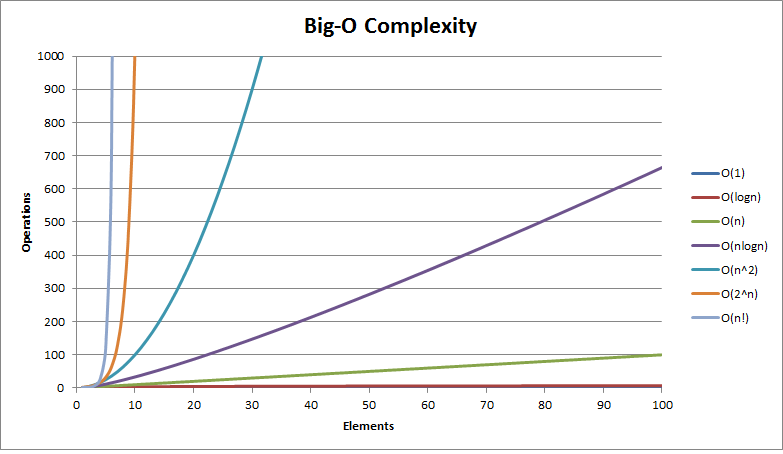
\includegraphics[width=0.75\textwidth]{images/big-o-complexity}\\
	Big-O Complexity comparison from ~\cite{bigocheatsheet}
\end{center}


\paragraph{Amdahl's Law.} One classic model of parallel execution
is Amdahl's Law. In 1967, Gene Amdahl argued that improvements in
processor design for single processors would be more effective than
designing multi-processor systems. Here's the argument. Let's say that
you are trying to run a task which has a serial part, taking fraction 
$S$, and a parallelizable part, taking fraction $P = 1-S$. Define $T_s$
to be the total 
amount of time needed on a single-processor system.
Now, moving to a parallel system with $N$ processors, the parallel
time $T_p$ is instead:
\[ T_p = T_s \cdot (S + \frac{P}{N}). \]
{\bf As $N$ increases, $T_p$ is dominated by $S$, limiting potential
speedup.}

We can restate this law in terms of speedup, which is the 
original time $T_s$ divided by the sped-up time $T_p$:
\[ \mbox{speedup} = \frac{T_s}{T_p} = \frac{1}{S+P/N}. \]
Replacing $S$ with $(1-P)$, we get:
\[ \mbox{speedup} = \frac{1}{(1-P)+P/N}, \]
and
\[ \mbox{max speedup} = \frac{1}{(1-P)}, \]
since $\frac{P}{N} \rightarrow 0$.

\paragraph{Plugging in numbers.} If $P = 1$, then we can indeed get good
scaling; running on an $N$-processor machine will give you a speedup
of $N$. Unfortunately, usually $P < 1$.  Let's see what happens.

\begin{center}
\begin{tabular}{r|r}
$P$ & speedup ($N=18$) \\ \hline
1 & 18 \\
0.99 & $\sim$ 15 \\
0.95 & $\sim$ 10 \\
0.5 & $\sim$ 2
\end{tabular}
\end{center}
Graphically, we have something like this:
\begin{center}
  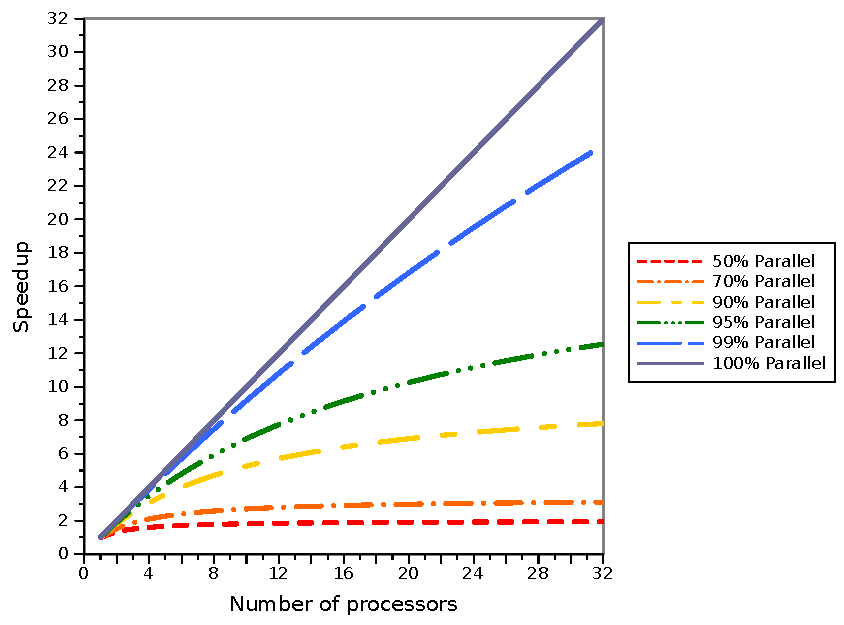
\includegraphics[width=0.5\textwidth]{images/parallel-scaling}
\end{center}


Amdahl's Law tells you how many cores you can hope to leverage in an
execution given a fixed problem size, if you can estimate $P$.

Let us consider an example from~\cite{mte241}: Suppose we have a task that can be executed in 5~s and this task contains a loop that can be parallelized. Let us also say initialization and recombination code in this routine requires 400~ms. So with one processor executing, it would take about 4.6~s to execute the loop. If we split it up and execute on two processors it will take about 2.3~s to execute the loop. Add to that the setup and cleanup time of 0.4~s and we get a total time of 2.7~s. Completing the task in 2.7~s rather than 5~s represents a speedup of about~46\%. Applying the formula, we get the following run times:

\begin{center}
	\begin{tabular}{l|l}
	\textbf{Processors} & \textbf{Run Time (s)} \\ \hline
	1 & 5\\
	2 & 2.7\\
	4 & 1.55\\
	8 & 0.975\\
	16 & 0.6875 \\
	32 & 0.54375 \\
	64 & 0.471875 \\
	128 & 0.4359375\\
	\end{tabular}
\end{center}

   \paragraph{Empirically estimating parallel speedup $P$.}
Assuming that you know things that are actually really hard to know, here's a formula for estimating speedup. You don't have to commit it to memory:
  \[P_{\mbox{\scriptsize estimated}} = \frac{\frac{1}{\mbox{\em speedup}}-1}{\frac{1}{N}-1}.\]

It's just an estimation, but you can use it to guess the fraction of parallel code, given $N$ and the speedup. You can then use $P_{\mbox{\scriptsize estimated}}$ to predict speedup for a different number of processors.

\paragraph{Consequences of Amdahl's Law.}
For over 30 years, most performance gains did indeed come from
increasing single-processor performance. The main reason that we're
here today is that, as we saw last time,
single-processor performance gains have hit the wall.

By the way, note that we didn't talk about the cost of synchronization
between threads here. That can drag the performance down even more.

\paragraph{Amdahl's Assumptions.}
Despite Amdahl's pessimism, we still all have multicore computers today.
Why is that? Amdahl's Law assumes that:
\begin{itemize}[noitemsep]
    \item problem size is fixed (read on);
    \item the program, or the underlying implementation, behaves the same on 1 processor as on $N$ processors; and
    \item that we can accurately measure runtimes---i.e. that overheads don't matter.
\end{itemize}

% replace Amdahl's law with how branch predictors work
\paragraph{Generalizing Amdahl's Law.} We made a simplification,
which was that programs only have one parallel part and one serial part.
Of course, this is not true. The program may have many parts,
 each of which we can tune to a different degree.

Let's generalize Amdahl's Law:

\begin{itemize}
\item  $f_1, f_2, \ldots, f_n$: fraction of time in part $n$
\item  $S_{f_1}, S_{f_n}, \ldots, S_{f_n}$: speedup for part $n$
\end{itemize}

Then,
\[\mbox{\em speedup} = \frac{1}{\frac{f_1}{S_{f_1}} + \frac{f_2}{S_{f_2}} + \ldots +
     \frac{f_n}{S_{f_n}}}.\]

\paragraph{Example.} Consider a program with 4 parts in the following scenario:

\begin{center}
     \begin{tabular}{r|r|r|r}
     \multicolumn{2}{l}{} & \multicolumn{2}{|c}{Speedup} \\
     Part & Fraction of Runtime & Option 1 & Option 2\\
     \hline
     1 & 0.55 & 1  & 2\\
     2 & 0.25 & 5  & 1\\
     3 & 0.15 & 3  & 1\\
     4 & 0.05  & 10 & 1\\
     \end{tabular}
 \end{center}

     (Note: these speedups don't have to be speedups from parallelization.)
    
   We can implement either Option 1 or Option 2. 
   Which option is better?

   ``Plug and chug'' the numbers:
 \begin{itemize}
 \item  {\bf Option 1.}

   \[ \mbox{\em speedup} = \frac{1}{0.55 + \frac{0.25}{5} + \frac{0.15}{3} + \frac{0.05}{5}}
     = 1.53  \]

 \item  {\bf Option 2.}

   \[\mbox{\em speedup} = \frac{1}{\frac{0.55}{2} + 0.45} = 1.38 \hspace*{5.5em}\]
\end{itemize}

\subsection*{A more optimistic point of view}
In 1988, John Gustafson pointed
out\footnote{\url{http://www.scl.ameslab.gov/Publications/Gus/AmdahlsLaw/Amdahls.html}}
that Amdahl's Law only applies to fixed-size problems, but that the
point of computers is to deal with bigger and bigger problems.

In particular, you might vary the input size, or the grid resolution,
number of timesteps, etc. When running the software, then, you might
need to hold the running time constant, not the problem size: you're
willing to wait, say, 10 hours for your task to finish, but not 500
hours. So you can change the question to: how big a problem can you
run in 10 hours?

According to Gustafson, scaling up the problem tends to increase the
amount of work in the parallel part of the code, while leaving the
serial part alone. As long as the algorithm is linear, it is possible
to handle linearly larger problems with a linearly larger number of
processors.

Of course, Gustafson's Law works when there is some ``problem-size''
knob you can crank up.  As a practical example, observe Google, which
deals with huge datasets.


\section*{Software Design Issues: Will it Parallelize?}


\paragraph{Locking and Synchronization Points.}
Think back to a concurrency course and the discussion of locking. We'll be coming back to this subject before too long. But for now, suffice it to say, that the more locks and locking we need, the less scalable the code is going to be. You may think of the lock as a resource and the more threads or processes that are looking to acquire that lock, the more ``resource contention'' we have, and the more waiting and coordination are going to be necessary. We're going to revisit the subject of wise use locks in more detail soon.

The previous paragraph applies as well to other concurrency constructs like semaphores, condition variables, etc. Any time a thread is forced to wait is going to be a limitation on the ability to parallelize the problem.

\paragraph{Memory Allocators.}
Assuming we're not working with an embedded system where all memory is statically allocated in advance, there will be dynamic memory allocation. The memory allocator is often centralized and may support only one thread allocating or deallocating at a time. This means it does not necessarily scale very well. There are, however, some techniques for dynamic memory allocation that allow these things to work in parallel.

\paragraph{Overhead.}
A first implementation might involve starting a thread for a task, then destroying it when it is complete. If there are many tasks and tasks are short-lived, then the fraction of time creating and destroying the threads may be significant.

 But that's not the only way. We can have a pool of workers. The workers are created once and only once. Then the application just submits units of work, and then on the other side these units of work are allocated to workers. The number of workers will scale based on the available hardware. This is neat as a programming practice: as the application developer we don't care quite so much about the underlying hardware. Let the operating system decide how many workers there should be, to figure out the optimal way to process the units of work.
 
Suppose you have to decide, though, how many threads should you create.
This depends
on which resources your threads use; if you are writing
computationally-intensive threads, then you probably want to have
fewer threads than the number of virtual CPUs. You can also use
Amdahl's Law to estimate the maximum useful number of threads, as
discussed previously.

Here's a longer discussion of thread pools:

\begin{center}
\url{http://www.ibm.com/developerworks/library/j-jtp0730.html}
\end{center}

Modern languages provide thread pools; Java's
\url{java.util.concurrent.ThreadPoolExecutor}~\cite{java:threadpoolexecutor}, C\#'s
\url{System.Threading.ThreadPool}~\cite{csharp:threadpool}, and GLib's {\tt GThreadPool}~\cite{gnome:threadpool} all implement thread pools. There's a Rust crate called \texttt{thread pool}. You can obviously write your own.

Here's a quick Rust program in which we use the threadpool crate to take away some of the complexity.
\begin{lstlisting}[language=Rust]
use std::collections::VecDeque;
use std::sync::{Arc, Mutex};
use threadpool::ThreadPool;
use std::thread;

fn main() {
    let pool = ThreadPool::new(8);
    let queue = Arc::new(Mutex::new(VecDeque::new()));
    println!("main thread has id {}", thread_id::get());

    for j in 0 .. 4000 {
        queue.lock().unwrap().push_back(j);
    }
    queue.lock().unwrap().push_back(-1);

    for i in 0 .. 4 {
        let queue_in_thread = queue.clone();
        pool.execute(move || {
            loop {
                let mut q = queue_in_thread.lock().unwrap();
                if !q.is_empty() {
                    let val = q.pop_front().unwrap();
                    if val == -1 {
                        q.push_back(-1);
                        println!("Thread {} got the signal to exit.", thread_id::get());
                        return;
                    }
                    println!("Thread {} got: {}!", thread_id::get(), val);
                }
            }
        });
    }
    pool.join();
}
\end{lstlisting}

It's important to note that when we call the \texttt{execute} function, that is a job to be run, so if our thread pool has four workers we want to push the consume ``job'' on it four times. They will then run and each will try to consume numbers until they get to the -1 answer which is the termination signal.

If we wrote our own implementation where we spawned the threads using the spawn mechanism, joining each thread individually might be a bit of a pain. 

This produces output that looks like:

\begin{verbatim}
main thread has id 4455538112
Thread 123145474433024 got: 0!
Thread 123145474433024 got: 1!
Thread 123145474433024 got: 2!

...

Thread 123145478651904 got: 3997!
Thread 123145478651904 got: 3998!
Thread 123145478651904 got: 3999!
Thread 123145476542464 got the signal to exit.
Thread 123145484980224 got the signal to exit.
Thread 123145474433024 got the signal to exit.
Thread 123145478651904 got the signal to exit.
\end{verbatim}

\paragraph{Threads and CPUs.} In your operating systems class,
you've seen implementations of threads (``lightweight processes'').
We'll call these threads \emph{software threads}, and we'll program
with them throughout the class. Each software thread corresponds to a
stream of instructions that the processor executes. On a old-school
single-core, single-processor machine, the operating system
multiplexes the CPU resources to execute multiple threads
concurrently; however, only one thread runs at a time on the single
CPU.

On the other hand, a modern chip contains a number of \emph{hardware
threads}, which correspond to the virtual CPUs. These are sometimes
known as \emph{strands}. The operating system still needs to 
multiplex the software threads onto the hardware threads, but now has
more than one hardware thread to schedule work onto.





\section*{Choose Your Pain}
The first design decision that you need to solve when parallelizing programs
is whether you should use threads or processes. Threads are basically light-weight processes which piggy-back on
          processes' address space.

\paragraph{When processes are better.} Processes are safer and more secure than threads.

  \begin{enumerate}
    \item Each process has its own virtual address space:
      \begin{itemize}
        \item Memory pages are not copied, they are copy-on-write (usually in UNIX, anyway). Therefore, processes use less memory than you would expect.
      \end{itemize}
    \item Buffer overruns or other security holes do not expose other~processes.
    \item If a process crashes, the others can continue.
  \end{enumerate}

{\bf Example:} In the Chrome browser, each tab is a separate
process. Scott McCloud explained this:
\url{http://www.scottmccloud.com/googlechrome/}.

\paragraph{When threads are better.} Threads are easier and faster.

  \begin{enumerate}
    \item Interprocess communication (IPC) is more complicated and slower than interthread
          communication; must use operating system utilities (pipes, semaphores, shared
              memory, etc) which have system call overhead, instead of Rust communication's mechanisms (shared memory or message passing)
	\item Processes have much higher startup, shutdown, and synchronization costs than threads.
  \end{enumerate}

\paragraph{How to choose?}
  If your application is like this:
  \begin{itemize}
    \item mostly independent tasks, with little or no communication;
    \item task startup and shutdown costs are negligible compared to overall runtime; and
    \item want to be safer against bugs and security holes,
  \end{itemize}
then processes are the way to go. If it's the opposite of this, then use threads.

For performance reasons, along with ease and consistency across systems, we'll use threads.

\paragraph{Overhead.} The common wisdom is that processes are
expensive, threads are cheap. Let's try it.

\begin{multicols}{2}

\begin{lstlisting}[language=Rust]
use std::process::Command;

fn main() {
    for j in 0 .. 50000 {
       Command::new("/bin/false").spawn();
    }
}
\end{lstlisting}
\begin{verbatim}
1.530 s +/-  0.134 s
\end{verbatim}
\columnbreak
\begin{lstlisting}[language=Rust]
use std::thread;

fn main() {
    for j in 0 .. 50000 {
        thread::spawn(|| {
            false
        });
    }
}
\end{lstlisting}
\begin{verbatim}
630.5 ms +/-  21.5 ms 
\end{verbatim}

\end{multicols}


\subsection*{Parallelization using Threads or Processes}
We'll be looking at thread-based or process-based parallelization for the
next bit. We don't care about the distinction between threads and processes
for the moment. In fact, we could even distribute work over multiple systems. But the idea is, if you are looking to parallelize your program, you should think about which of the following patterns makes the most sense.

\paragraph{Pattern 1: Multiple Independent Tasks.} If you're just trying to maximize
system utilization, you can use one system to run a number of independent
tasks; for instance, you can put both a web server and database on
one machine. If the web server happens to be memory-bound while the
database is I/O-bound, then both can use system resources. If the web
server isn't talking to the database (rare these days!), then the tasks
would not get in each others' way.

Most services probably ought to be run under virtualization these
days, unless they're trivial or not mission-critical.

A more relevant example of multiple independent tasks occurs in
cluster/grid/cloud computing: the cloud might run a number of
independent tasks, and each node would run some of the tasks. The
cloud can retry a task (on a different node, perhaps) if it fails on
some node. Note that the performance ought to increase linearly with
the number of threads, since there shouldn't be communication between
the tasks.

\paragraph{Pattern 2: Multiple Loosely-Coupled Tasks.} Some applications contain
tasks which aren't quite independent (so there is some inter-task
communication), but not much.  In this case, the tasks may be
different from each other. The communication might be from the tasks
to a controller or status monitor; it would usually be asynchronous or
be limited to exceptional situations.

Refactoring an application this way can help with latency: if you 
split off the CPU-intensive computations into a sub-thread, then
the main thread can respond to user input more quickly.

Here's an example. Assume that an application needs to receive and
forward network packets, and also must log packet activity to disk.
Then the two tasks are clear: receive/forward, and log. Since logging
to disk is a high-latency event, a single-threaded application might
incur latency while writing to disk. Splitting into subtasks allows
the receive/forward to run without waiting for previous packets to be
logged, thus increasing the throughput of the system.

\paragraph{Pattern 3: Multiple Copies of the Same Task.} A common variant of
multiple independent tasks is multiple copies of the same task
(presumably on different data). In this case, we'd require there to be
no communication between the different copies, which would enable
linear speedup. An example is a rendering application running on
multiple distinct animations. We gain throughput, but need to wait
just as long for each task to complete.

\paragraph{Pattern 4: Single Task, Multiple Threads.} This is the classic
vision of ``parallelization'': for instance, distribute array
processing over multiple threads, and let each thread compute the
results for a subset of the array.

This pattern, unlike many of the others before it, can actually
decrease the time needed to complete a unit of work, since it gets
multiple threads involved in doing the single unit simultaneously.
The result is improved latency and therefore increased throughput.
Communication can be a problem, if the data is not nicely
array-structured, or has dependencies between different array parts.

Other names and variations for this pattern include ``fork-join'',
where the main process forks its execution and gives work to all of
the threads, with the join synchronizing threads and combining the
results; and ``divide-and-conquer'', where a thread spawns subthreads
to compute smaller and smaller parts of the solution.

\paragraph{Pattern 5: Pipeline of Tasks.} We've seen pipelining in the context of
computer architecture. It can also work for software. For instance,
you can use pipelining for packet-handling software, where multiple
threads, as above, might confound the order. If you use a three-stage
pipeline, then you can have three packets in-flight at the same time,
and you can improve throughput by a factor of 3 (given appropriate
hardware).  Latency would tend to remain the same or be worse (due to
communication overhead).

Some notes and variations on the pipeline: 1) if a stage is
particularly slow, then it can limit the performance of the entire
pipeline, if all of the work has to go through that stage; and 2) you
can duplicate pipeline stages, if you know that a particular stage is
going to be the bottleneck.

\paragraph{Pattern 6: Client-Server.} Botnets work this way (as does \verb+SETI@Home+,
etc). To execute some large computation, a server is ready to tell
clients what to do.  Clients ask the server for some work, and the
server gives work to the clients, who report back the results. Note
that the server doesn't need to know the identity of the clients for
this to work.

A single-machine example is a GUI application where the server part
does the backend, while the client part contains the user interface.
One could imagine symbolic algebra software being designed that way.
Window redraws are an obvious candidate for tasks to run on clients.

Note that the single server can arbitrate access to shared resources.
For instance, the clients might all need to perform network access.
The server can store all of the requests and send them out in an
orderly fashion.

The client-server pattern enables different threads to share work
which can somehow be parcelled up, potentially improving
throughput. Typically, the parallelism is somewhere between single
task, multiple threads and multiple loosely-coupled tasks. It's also a
design pattern that's easy to reason about.

\paragraph{Pattern 7: Producer-Consumer.} The producer-consumer is 
a variant on the pipeline and client-server models. In this case, the
producer generates work, and the consumer performs work. An example is
a producer which generates rendered frames, and a consumer which
orders these frames and writes them to disk. There can be any number
of producers and consumers. This approach can improve throughput
and also reduces design complexity.

\paragraph{Combining Strategies.} If one of the patterns suffices,
then you're done. Otherwise, you may need to combine strategies.
For instance, you might often start with a pipeline, and then 
use multiple threads in a particular pipeline stage to handle one
piece of data. Or, as I alluded to earlier, you can replicate
pipeline stages to handle different data items simultaneously.

Note also that you can get synergies between different patterns.
For instance, consider a task which takes 100 seconds. First, you
take 80 seconds and parallelize it 4 ways (so, 20 seconds). This
reduces the runtime to 40 seconds. Then, you can take the serial 
20 seconds and split it into two threads. This further reduces 
runtime to 30 seconds. You get a $2.5\times$ speedup from the
first transformation and $1.3\times$ from the second, if you do it
after the first. But, if you only did the second parallelization,
you'd only get a $1.1\times$ speedup.


\bibliographystyle{alphaurl}
\bibliography{459}


\end{document}
